\section{Dataset analysis}

\subsection{Dataset presentation and modifications}

\subsubsection{Dataset presentation.}

We focus on two datasets. The first one is PEPSI, a compilation of synthetic flow observations generated from outputs of various hydraulic flow models. This dataset is composed of 55525 observations from 29 rivers worldwide, with 21 explanatory variables for each of them. The second dataset, HydroSwot is generated from observations -- from 153 rivers -- taken in-situ in North America. It contains 16638 observations with 41 explanatory variables. Table \ref{tab:varaibles} describes the explanatory variables contained in both datasets, and that we use for the statistic analysis.


\begin{table}[H]
    \centering
    \begin{tabular}{|c|c|c|c|}
    \hline
        Variable & Description & HydroSwot & PEPSI  \\ \hline \hline
        river &  river name & X & X \\ \hline
        site\_no & site number & X & \\ \hline
        day & simulation day & & X \\ \hline
        reach & reach index & &X \\ \hline
        reach\_length & length of the reach & & X \\ \hline 
        flowacc & flow accumulation, i.e. size of the upstream watershed & X & X \\ \hline
        height & free surface height & X & X \\ \hline 
        dH & water depth above unobserved flow & X & \\ \hline
        W &  free surface top width & X & X \\ \hline
        S & free surface slope  &  & X \\ \hline
        Sdem & terrain slope & X & \\ \hline
        K & Strickler value & & X \\ \hline
        Fr & Froude number & & X \\ \hline
        \alpha, \beta & Manning-Strickler coefficients & & X \\ \hline 
        A & cross-section flow area & & X \\ \hline 
        dA & cross-sectional flow area above A0 & X & X \\ \hline
        A0 & unobserved cross-sectional flow area & X & X\\ \hline
        Abar & mean cross-sectional flow area  data & X & X\\ \hline
        Amed & median cross-sectional flow area  data & X & \\ \hline
        U & flow velocity & X & X\\ \hline
        Q & discharge & X & X \\ \hline
        PA & mean annual precipitation & X & \\ \hline
        TA & mean annual temperature & X & \\ \hline
        sinuosity & sinuosity & & X \\ \hline 
        meandwave & meandering wavelenght & & X \\ \hline 
        Sand, salt, ... & floor composition & X &X \\ \hline 
        lon, lat & localisation & X & X \\ \hline 
        LC1, LC2, ... & vegetation information & X & \\ \hline 
        
    \end{tabular}
    \caption{Explanatory variables of HydroSwot and PEPSI datasets}
    \label{tab:varaibles}
\end{table}
\underline{Remark:} the values of the river discharge $Q$ have an uncertainty of 20\%. 


\subsubsection{Dataset modifications.\label{section212}}

First, we clean our datasets. We delete all observations with $NaN$ values, i.e. missing values. In the HydroSwot dataset, we can find different names for the same river because of text processing when creating the data. We update the names to have each river with a single name and make easier the analysis. We obtain 134 rivers.

The satellite does not detect small rivers with a width less than $80m$. Thus, we delete observations with a width under $80m$. We also remove observations with a river discharge under $100 m^3/s$ because we assume they are too precise observations, and so they do not have a real meaning.

We remove the calculations of base streamflow, and the different mean discharge quantile from the HydroSwot dataset. We also remove the flow velocity $U$ in the two datasets, because $U$ is linearly linked to $Q$ according to the following equation : $Q = AU$.\newline

Finally, we obtain a dataset with 29 rivers, 51269 observations, and 20 variables for PEPSI, and a dataset with 134 rivers, 11851 observations, and 21 variables for HydroSwot.
        
Due to previous modifications, we obtain only 1 observation for 8 sites in the HydroSwot dataset. We cannot use these data because the variables $dA$ and $dH$ are calculated by differences, so we must have at least 2 observations to give them meaning. Hence, we remove these 8 observations. To conclude, we lose 29\% of data in the HydroSwot dataset and 8\% in the PEPSI dataset.

\subsection{Statistical methods}

\subsubsection{Correlation matrix.}

We seek to determine which variables are related. 

The correlation is the relationship between two random quantitative variables which explains how they are linearly related. It is defined by :
\begin{equation}
    Cor(\underline{x},\underline{y}) = \frac{Cov(\underline{x},\underline{y})}{\sqrt{Var(\underline{x})Var(\underline{y})}}
\end{equation}
where \underline{x} and \underline{y} denote the samples of the two variables, $Cov$ the covariance between them, and $Var$ their respective variance. The correlation varies between $-1$ when the variables vary in strong opposite directions, and $1$ when they vary exactly in the same direction. Here, we use a correlation matrix to easily summarise all the correlations between all variables : one cell of the matrix represents the correlation between the row variable and the column one. Thus, the diagonal is full of $1$s, as it represents the correlation between a variable and itself.\newline

\subsubsection{Principal Component Analysis.}

The goal of  a Principal Component Analysis (PCA) (Wikistat, 2016 \cite{ACP}) is to reduce the large shape of our problem by gathering our variables within metavariables to analyse our data more easily. The first step consists in a normalization of the data because of the different scales (understand units) of our variables. Then, we compute linear combinations of our initial variables. One linear combination represents one principal component or direction. The aim is to find which direction maximises the amount of variance of the data, i.e. the direction that captures most information of the data. 

Let $\Sigma$ be the covariance matrix associated to the normalized data. Computing the principal component involves determining the eigenvector $a_1$ associated to the largest eigenvalue of $\Sigma$ denoted as $\lambda_1$, i.e. to solve the following equation :
\begin{equation}
    \Sigma a_1 = \lambda_1 a_1
\end{equation}
Thus, we get the principal components by order of significance by ranking the eigenvectors according to the values of their associated eigenvalues. Then, we select the number of axes which is necessary to capture the majority of the information. A well-known rule is to keep the first $n$ components such as the sum of their variances reaches $80\%$ of the total variance.

Finally, we interpret our PCA with two different types of graph. The first one is the loading plot: all the variables of the problem are displayed in the spans formed by each pair of principal components retained. The aim is to find how the initial variables are related with the principal components. The second plot is the score plot, which plots the individuals' coordinates in the the same spans as mentioned above. We then can observe clusters of individuals.

\subsubsection{Clustering by K-means.}

K-means is an unsupervised classification method to define clusters in a dataset. We first have to find the optimal number $k$ of clusters to give to the algorithm. Then, it works as follows.

First, $k$ class centers, called centroids, are randomly initialized. Second, individuals are assigned to the class whose center is closest, according to the chosen distance metric. Here, we use the Euclidean metric. It is defined as follows, for a pair of samples $a$ and $b$ $\in \mathbb{R}^n$:
\begin{equation}
    dist_{euc}(a,b) = \sqrt{\sum^n_{i=1} (a_i - b_i)^2}
\end{equation}

Third, the centers of gravity of each class are computed. Finally, we repeat second and third instructions until the convergence of the algorithm.

One advantage of the K-means algorithm is that we are certain to obtain a convergence of it. Nonetheless, we obtain different classes depending on the random initialization at the beginning. To overcome this problem, the algorithm will be run with different centroid seeds, and the final results will be the best output in terms of inertia.

\subsection{Variables selection \label{variables_selection}}
\subsubsection{Correlations with the river discharge.\label{section231}}

Despite the variables' removal done in the \nameref{section212} section, we still have too many variables in our datasets.
Thus, we need to reduce this number and to focus only on the essential variables. So we perform an advanced statistical analysis.

First, we calculate the correlation matrix and we focus on the most correlated variables with the river discharge $Q$ (see Figure \ref{fig:corH} and Figure \ref{fig:corP}).
\begin{figure}[H]
\centering
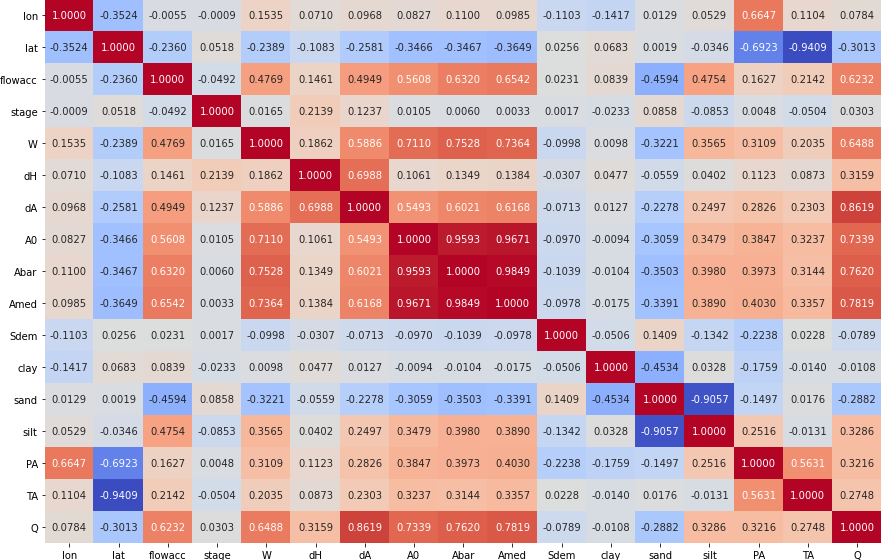
\includegraphics[scale=0.4]{Graph/correlation_hydro.png}
\caption{Correlation matrix of the HydroSwot dataset}
\label{fig:corH}
\end{figure}

For HydroSwot, we see in Figure \ref{fig:corH} that the highest coefficients of correlation with $Q$ are $dA$, $Abar$, $A0$, $Amed$, $W$, and $flowacc$. On the one hand, it makes sense to see $Abar$, $A0$, and $Amed$ so high because they are part of the equation to compute $Q$. On the other hand, $dA$, $W$, and $flowacc$ appear to be variables the most correlated with $Q$. In contrast, $Sdem$ is not highly correlated with $Q$.

\begin{figure}[H]
\centering
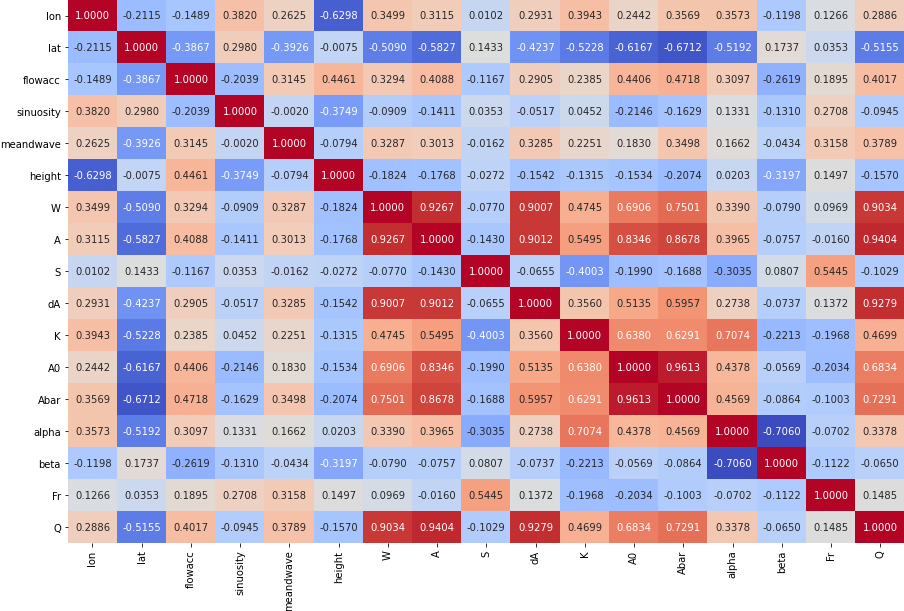
\includegraphics[scale=0.4]{Graph/correlation_pepsi.png}
\caption{Correlation matrix of the PEPSI dataset}
\label{fig:corP}
\end{figure}

For Pepsi, we calculate the correlations in figure \ref{fig:corP}. As for HydroSwot, we observe that $dA$ and $W$ are the two most correlated variables with the river discharge $Q$. But this time, $flowacc$ is much less correlated with $Q$, and the Strickler coefficient $K$ has a high coefficient correlation with $Q$.\newline

To conclude the analysis of the correlation coefficients, the most essential variables that explain $Q$ seem to be $dA$, $W$, and $flowacc$. We verify this conclusion with a Principal Component Analysis. 

\subsubsection{Principal Component Analysis.}

The first step of a PCA is to determine the number of principal components. Due to the high dimension of our datasets, the boxplot of the components is hardly sufficient to determine an optimal number of principal axes (see Figure \ref{fig:pcahydro} and Figure \ref{fig:pcapepsi}). 
 
 \begin{figure}[H]
     \centering
     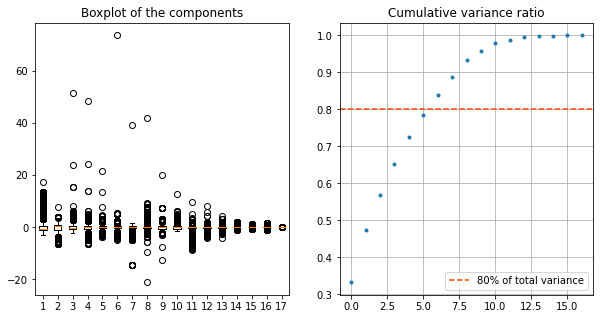
\includegraphics[scale = 0.55]{Graph/hydro_pca.png}
     \caption{Boxplot of the components and cumulative variance ratio plot, HydroSwot dataset}
     \label{fig:pcahydro}
 \end{figure}
 
Although we cannot determine the exact number of components using the boxplot, the plot of the cumulative variance ratio (see Figure \ref{fig:pcahydro}) shows that 6 components are sufficient to almost reach $80\%$ of the total variance for the HydroSwot dataset.

 \begin{figure}[H]
     \centering
     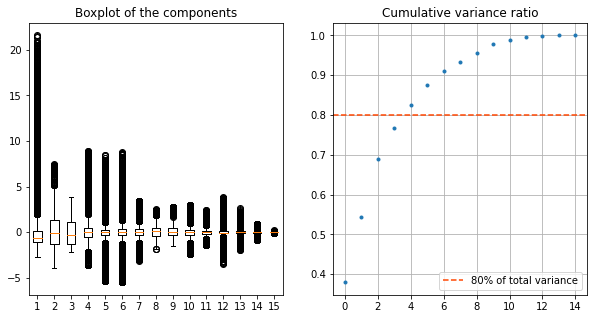
\includegraphics[scale = 0.55]{Graph/pepsi_pca.png}
     \caption{Boxplot of the components and cumulative variance ratio plot, PEPSI dataset}
     \label{fig:pcapepsi}
 \end{figure}

For the PEPSI dataset, 4 components seem to be sufficient. Taking a fifth principal component to reach $80\%$ of the total variance just represents a small ratio of variance, so we decide to take 4 principal axes.

Then, we show the loading plots. We want to find the major interactions, so we focus on the spans formed by the two first principal components (See Figure \ref{fig:factormap}).

\begin{figure}[H]
    \centering
    \begin{subfigure}{0.45\textwidth}
        \centering
        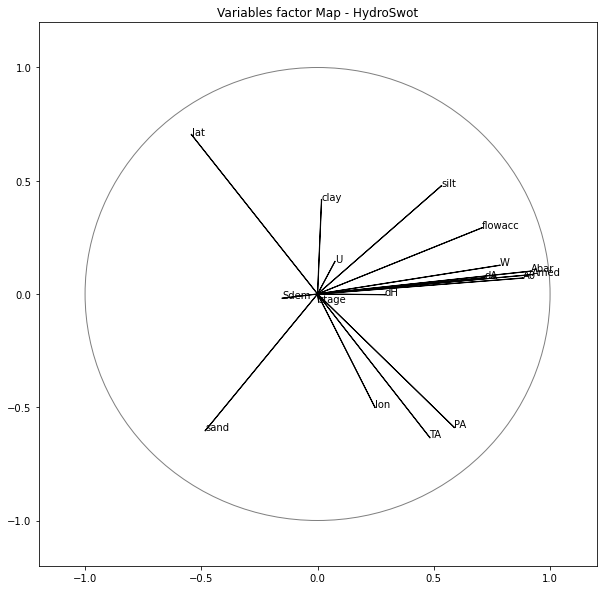
\includegraphics[scale=0.28]{Graph/factor_map_hydro.png}
        \caption{HydroSwot}
        \label{subfig:fmh}
    \end{subfigure}
    \begin{subfigure}{0.45\textwidth}
        \centering
        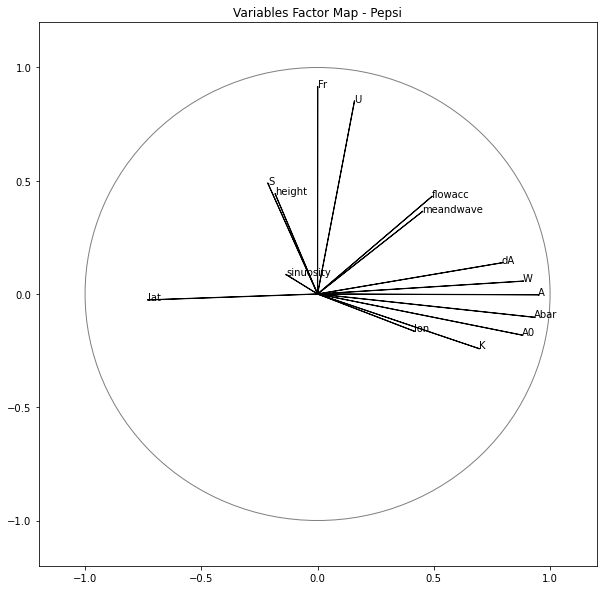
\includegraphics[scale=0.28]{Graph/factor_map_pepsi.png}
        \caption{PEPSI}
        \label{subfig:fmp}
    \end{subfigure}
\caption{Loading plots in the span formed by components 1 and 2}
\label{fig:factormap}
\end{figure}

As we can see on Figure \ref{subfig:fmh}, for HydroSwot, the variables that most explain the principal component are $dA$, $W$, and $flowacc$, as the first two ones are almost parallel to the first axe. We also notice the importance of the composition of the river with $sand$ and $silt$, the meteorological data with $PA$ and $TA$, and finally the geographical position. 

As for HydroSwot, $dA$, $W$, and $flowacc$ are good descriptors of the first component of the PEPSI dataset (see Figure \ref{subfig:fmp}). This time, we observe that the slope $S$ is part of the significant variables. Once again, we observe the importance of the physical metric such as the Froude Number, $Fr$, and the Strickler coefficient, $K$.\newline

Finally, we display the score plots in the span formed by the two principal components (see Figure \ref{fig:scoreplot}).

\begin{figure}[H]
    \centering
    \begin{subfigure}{0.45\textwidth}
        \centering
        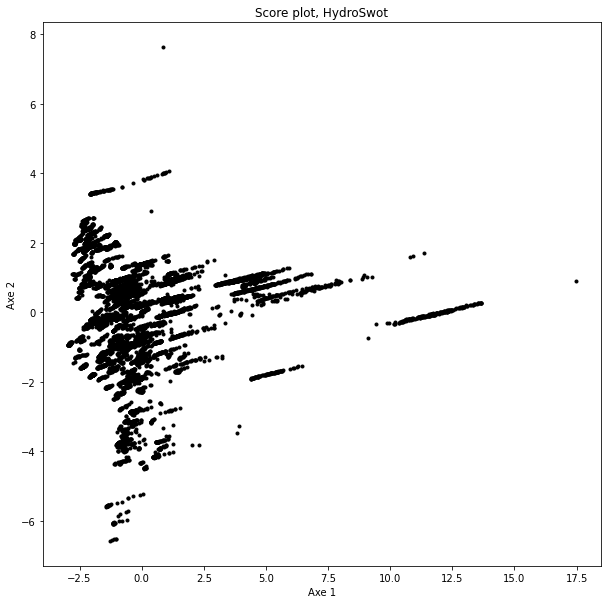
\includegraphics[scale=0.28]{Graph/scoreplot_hydro.png}
        \caption{HydroSwot}
        \label{subfig:sph}
    \end{subfigure}
    \begin{subfigure}{0.45\textwidth}
        \centering
        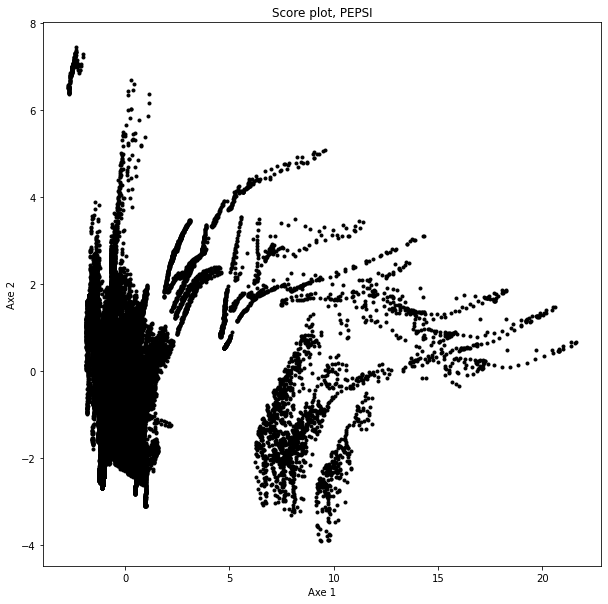
\includegraphics[scale=0.28]{Graph/scoreplot_pepsi.png}
        \caption{PEPSI}
        \label{subfig:spp}
    \end{subfigure}
\caption{Score plots in the span formed by components 1 and 2}
\label{fig:scoreplot}
\end{figure}

Concerning the HydroSwot dataset, we observe in Figure \ref{subfig:sph} that the individuals form lines whose directions are similar to the directions of $dA$, $W$, and $flowacc$ on the loading plot of HydroSwot (see Figure \ref{subfig:fmh}). It stresses the fact that these variables are very significant (see \nameref{section231} section) in this dataset, and it suggests that each line represents all the observations of a particular river.

We see in Figure \ref{subfig:spp} that the individuals from the PEPSI dataset have a singular representation, but it is difficult to analyse the meaning of it. Even so, we notice two different groups, that may correspond to two different scale of river discharge.\newline

To  summarise, the multidimensional analysis leads us to use four input variables for the neural networks : $W$, $dA$, $flowacc$, and the slope ($Sdem$ for HydroSwot, and $S$ for Pepsi, which seems to be more significant than $Sdem$).

\subsubsection{River Classification.\label{section233}} 

To have the most accurate flow estimation, we split rivers into groups. We need to define the number of groups and how to determine them.

We compute a K-means classification for the two datasets with 2 and 3 groups. More groups would lead to too small groups, i.e. with not enough observations to run neural networks algorithms. For both datasets, the K-means classification on 2 groups determines a huge group with the majority of the observations and the other with the rest of the observations. The K-means classification with 3 groups leads to 2 equivalent groups in size and the third group remains small.  

Figure \ref{fig:kmeans} shows a representation of classes by K-means for the HydroSwot dataset. We notice that K-means separates groups distinctly. It also suggests that observations from the same river can be in several groups. K-means classification does not separate rivers between them, it suggests to separate data by river portions.

\begin{figure}[H]
    \begin{subfigure}{0.45 \textwidth}
        \centering
        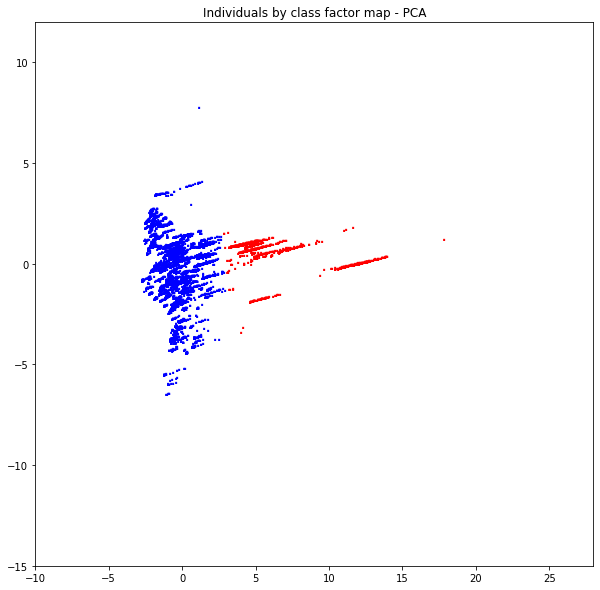
\includegraphics[scale = 0.3]{Graph/kmeans2HS.png}
        \caption{2 classes}
    \end{subfigure}
\centering
    \begin{subfigure} {0.45 \textwidth}
        \centering
        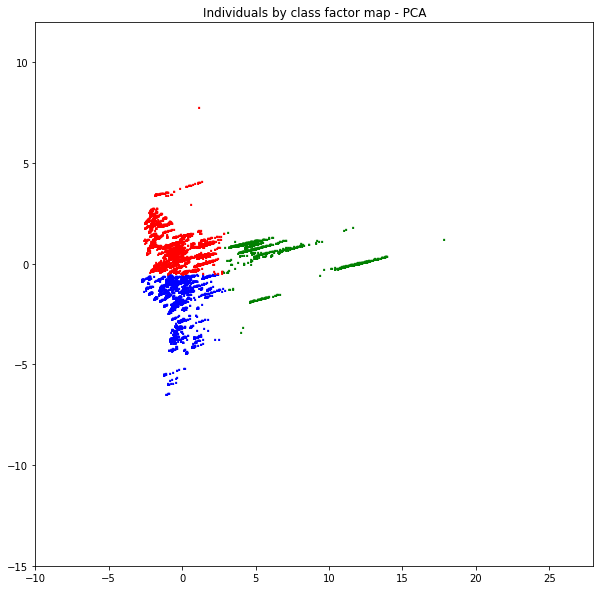
\includegraphics[scale = 0.3]{Graph/kmeans3HS.png}
        \caption{3 classes}
    \end{subfigure}
\caption{Plots for different numbers of classes in the span of the 2 first ACP components for Hydroswot }
\label{fig:kmeans}
\end{figure}

Splitting into 3 groups is not needed for our study. Indeed, we aim to have the largest dataset possible. 

We examine in figure \ref{fig:boxplot_hydro} boxplots of the different variables depending on groups determined by K-means for both datasets. We note that variables which distinct the 2 groups are mainly $Q$ and $flowacc$. $dA$ is also a good separator. \newline

\begin{figure}[H]
\begin{subfigure}{0.45\textwidth }
     \centering
        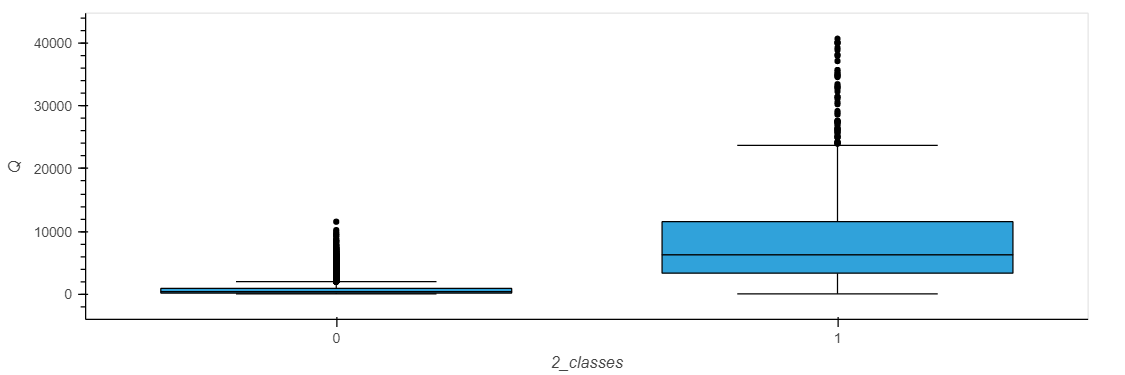
\includegraphics[scale = 0.19]{Graph/bokeh_plot.png}
        \caption{Boxplot of Q}
\end{subfigure}
\begin{subfigure}{0.45\textwidth}
     \centering
        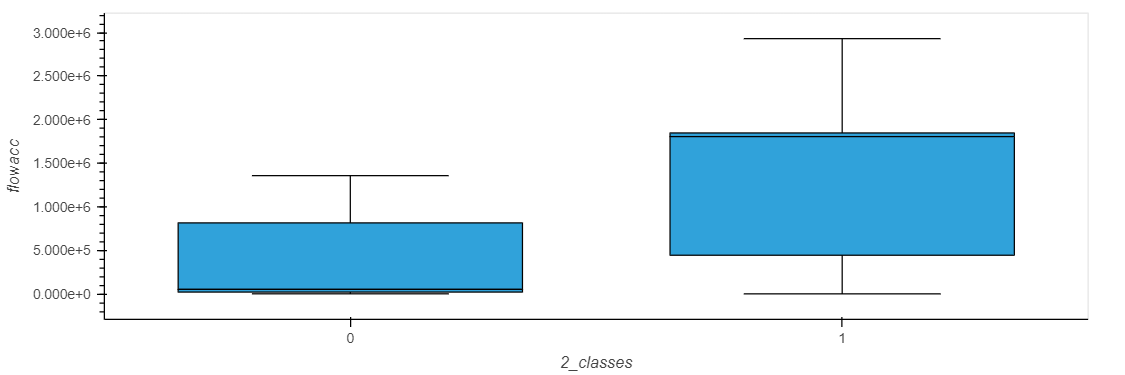
\includegraphics[scale = 0.19]{Graph/flowacc_hydro.png}
        \caption{Boxplot of flowacc }
\end{subfigure}
  \caption{Boxplots of different variables for 2 HydroSwot classes}     
  \label{fig:boxplot_hydro}
\end{figure}

\underline{Remark:} we do not show results of K-means classification for the PEPSI dataset because we obtain the same results and conclusions. \\
    
We finally choose two ways to separate rivers for both datasets. Each method separate rivers into 2 groups as we do not have enough data to create 3 groups.

First, we group data by rivers and compute the river flow mean. We separate them using the criteria of $Q$ which is a good separator according to K-means method. For HydroSwot, we make 2 groups: high discharge rivers ($Q > 1000 m^3/s$) and low discharge rivers ($Q < 1000 m^3/s$). For Pepsi we fix the boundary at $3000 m^3/s$. We notice that the high discharge rivers group for PEPSI contains only 3 rivers: $Mississipi$, $Padma$ and $Jamuna$. This separation by entire rivers is close to the real context of the SWOT Mission. For LSTM network, we will train and test on entire rivers that we know exactly. Then, we will use this algorithm on unknown rivers that the satellite would have measured. We name these separations Hydroswot/PEPSI Handmade - Low/High $Q$.\\

\underline{Remark :} we could separate the datasets using $flowacc$ as we saw that it is also a good separator. \\
The second way to separate data is by following K-means method to split Hydroswot and Pepsi into 2 classes. Among separative variables we have $Q$, so we decide to name the two classes with Low $Q$ and High $Q$. Thus, we obtain Table \ref{Tab:class_prop}.

\begin{table}[H]
\centering
    \begin{tabular}{|c|c|c|}
    \hline
    & Low $Q$ & High $Q$ \\ \hline
    Hydroswot Handmade & 6714 & 5129 \\\hline
    Pepsi Handmade & 47548 & 3721 \\\hline
    Hydroswot K-means  &  10490 & 1140 \\\hline
    Pepsi K-means & 47536 & 2674\\ \hline
    \end{tabular}
\caption{Number of observations in the different classes}
\label{Tab:class_prop}
\end{table}

We notice that HydroSwot K-means - High $Q$ has only 1140 observations. This small number may impact the efficiency of neural networks.
